%% appendix.tex
%%

%% ==============================
\Appendix
\label{ch:Appendix}
%% ==============================



\section{Technische Doku über die Benutzung von den MITK Segmentierungstools}

Als erstes muss in den DICOM Ordner der Ordner mit ungefähr 200 Elementen gefunden werden.

\begin{figure}[H] 
\centering 
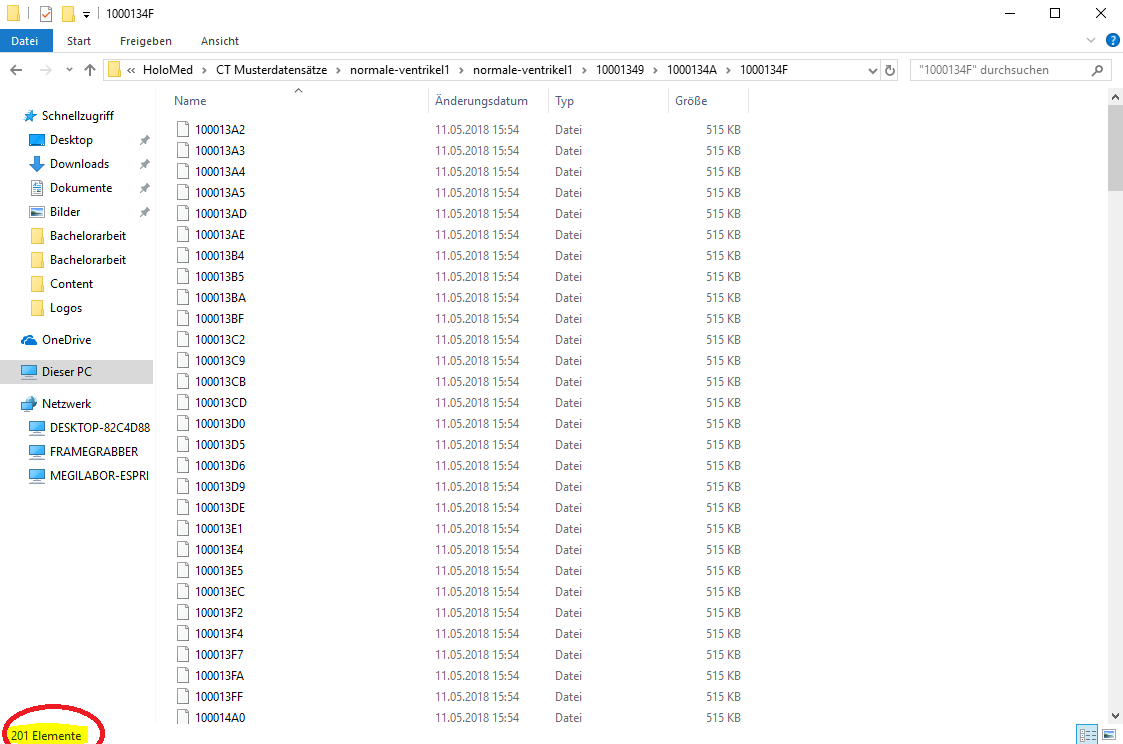
\includegraphics[width=0.7\textwidth]{Logos/MITK_Doku/1.PNG}
\caption{1} 
\label{fig:eins} 
\end{figure}

Anschließend kann eine der Dateien des Ordners via drag and drop in den \textit{Data Manager} gezogen werden und das Fenster das erscheint bestätigt werden.
\newline
Hier sieht man in der Mitte die verschiedenen Schnittbilder durch die man mit der Maus durchschauen kann.
\newline
Bei den Zahlen 1 bis 5 kann man die verschiedenen Tools sehen. Klickt man diese an öffnet sich an der Seite oder unter den Schnittbildern das jeweilige Tool. Möchte man ein Tool auf eine Datei anwenden, so muss die Datei stets im \textit{Data Manager} ausgewählt sein.
\newline
Mit dem Regler rechts am Rand der Schnittbilder kann die Darstellung der Grauwerte eingestellt werden.

\begin{figure}[H] 
\centering 
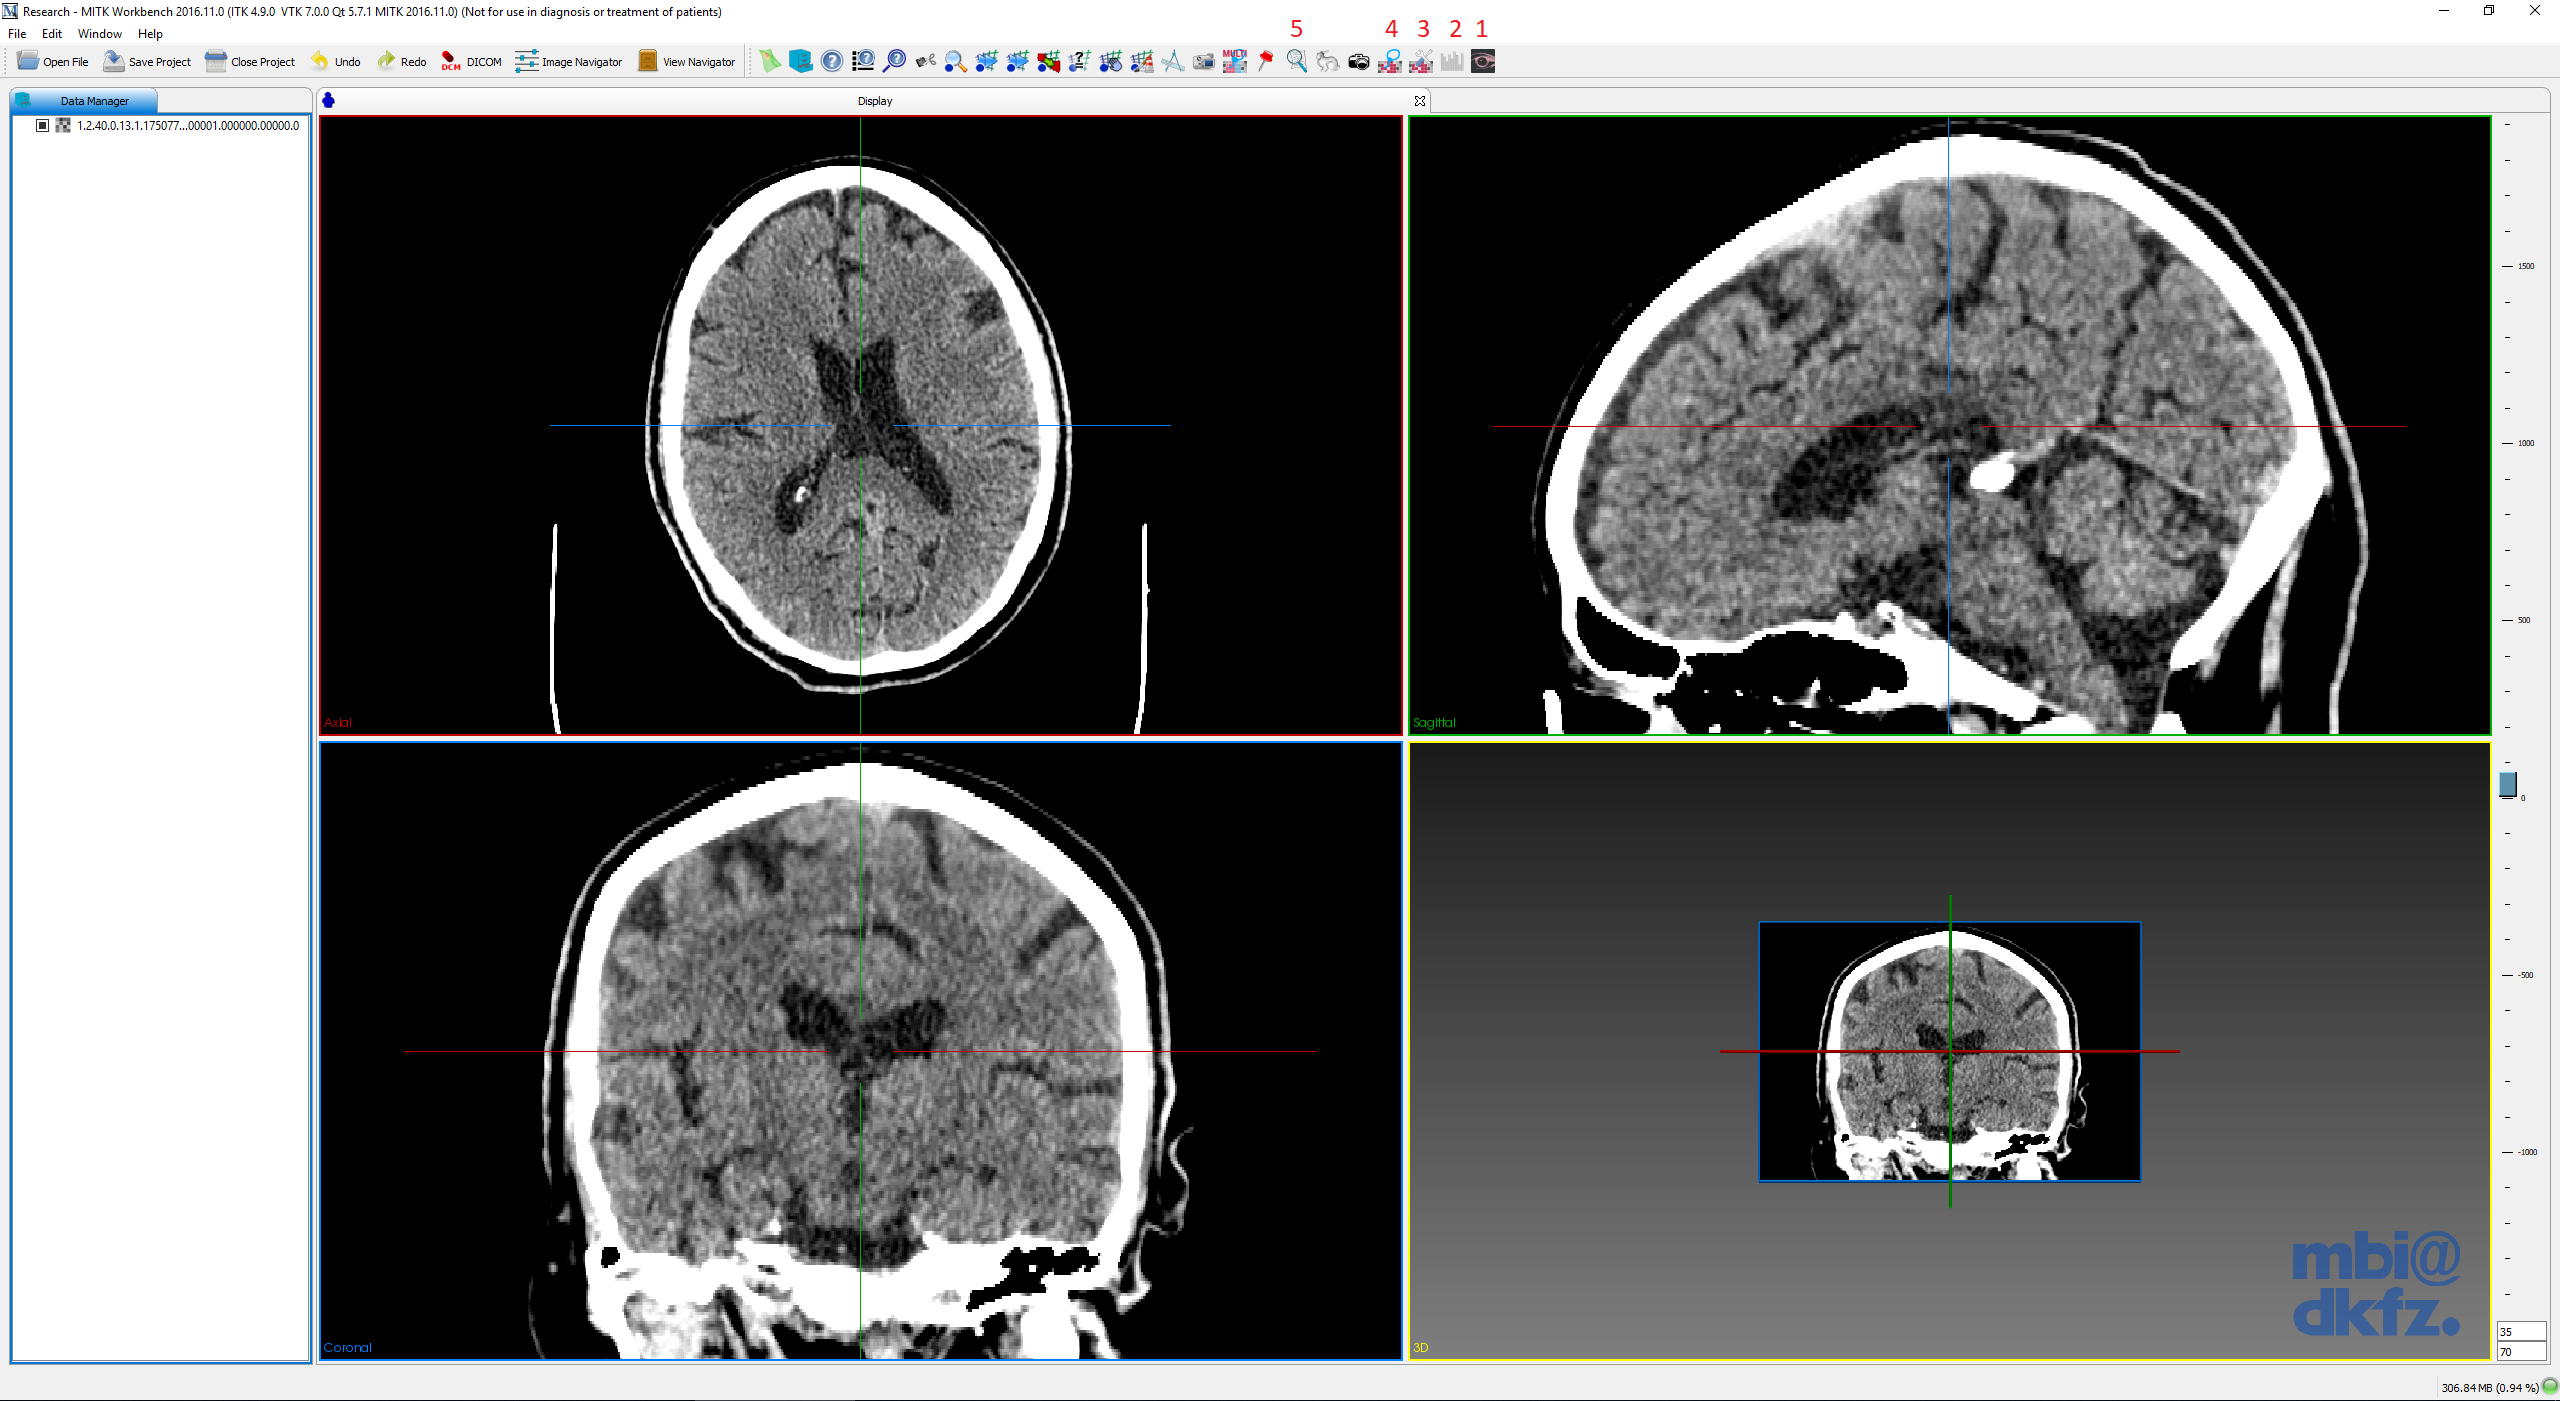
\includegraphics[width=\textwidth]{Logos/MITK_Doku/2.PNG}
\caption{2} 
\label{fig:zwei} 
\end{figure}

Das Tool mit der Nummer 1 macht es möglich eine Transferfunktion zu definieren. Anhand der Intensitätswerte, den Punkten über dem Diagramm und dem Farbstrahl darunter kann die Transferfunktion angepasst werden. setzt man den Haken bei \textit{Volumerendering} kann man im Fenster links unten die Visualisierung sehen.

\begin{figure}[H] 
\centering 
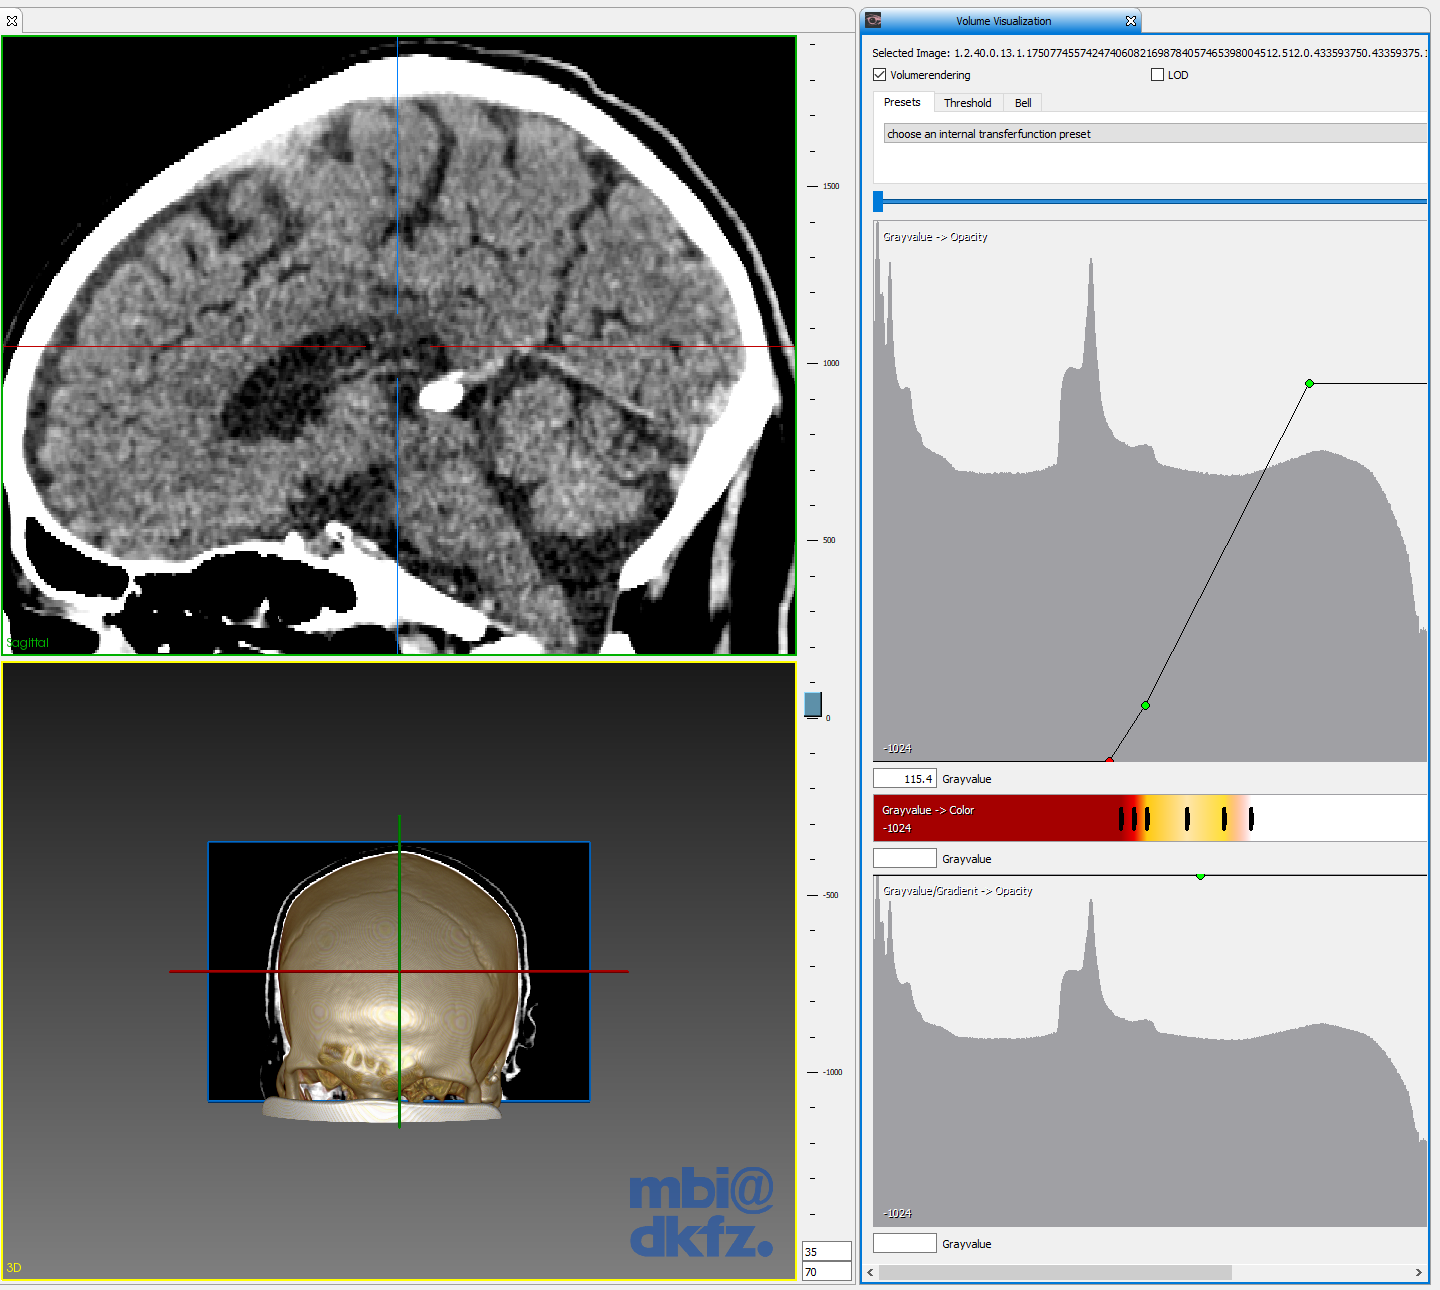
\includegraphics[width=0.7\textwidth]{Logos/MITK_Doku/3.PNG}
\caption{3} 
\label{fig:drei} 
\end{figure}

Das Tool mit der Nummer 2 zeigt Statistiken zum Volumen an, wie zum Beispiel Verteilung der Intensitätswerte, der Median dieser etc.

\begin{figure}[H] 
\centering 
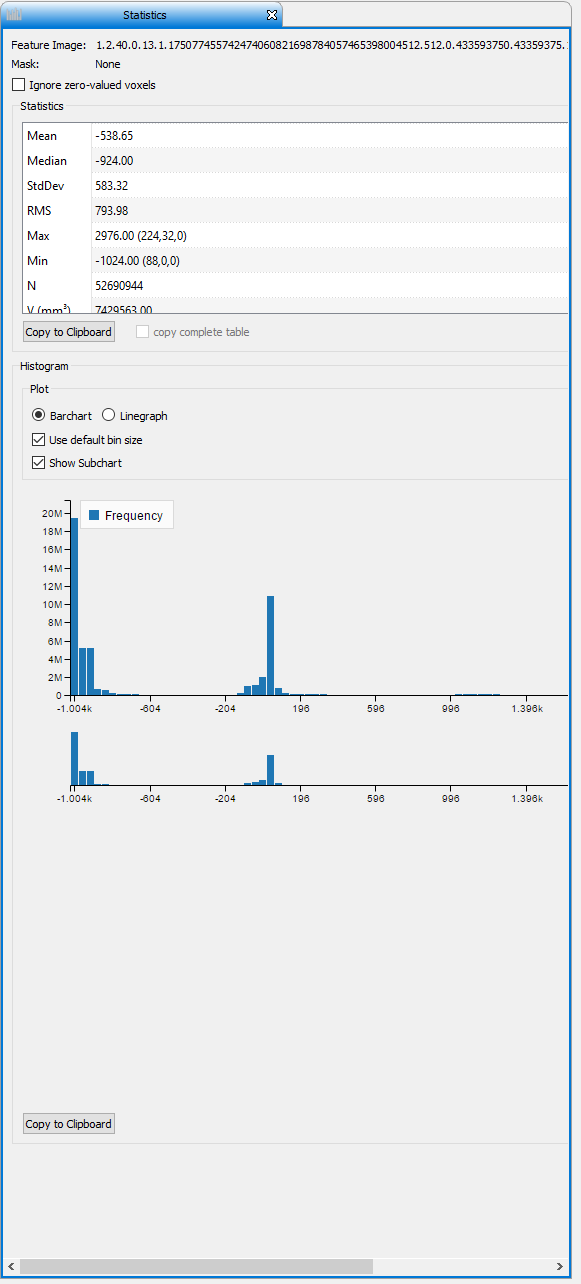
\includegraphics[width=0.4\textwidth]{Logos/MITK_Doku/4.PNG}
\caption{4} 
\label{fig:vier} 
\end{figure}

Das Tool Nummer 3  bietet verschiedene 2D und 3D Segmentierungstools an. Zunächst muss man doch eine neue Segmentierung über den rot markierten Knopf erstellen.

\begin{figure}[H]
\centering 
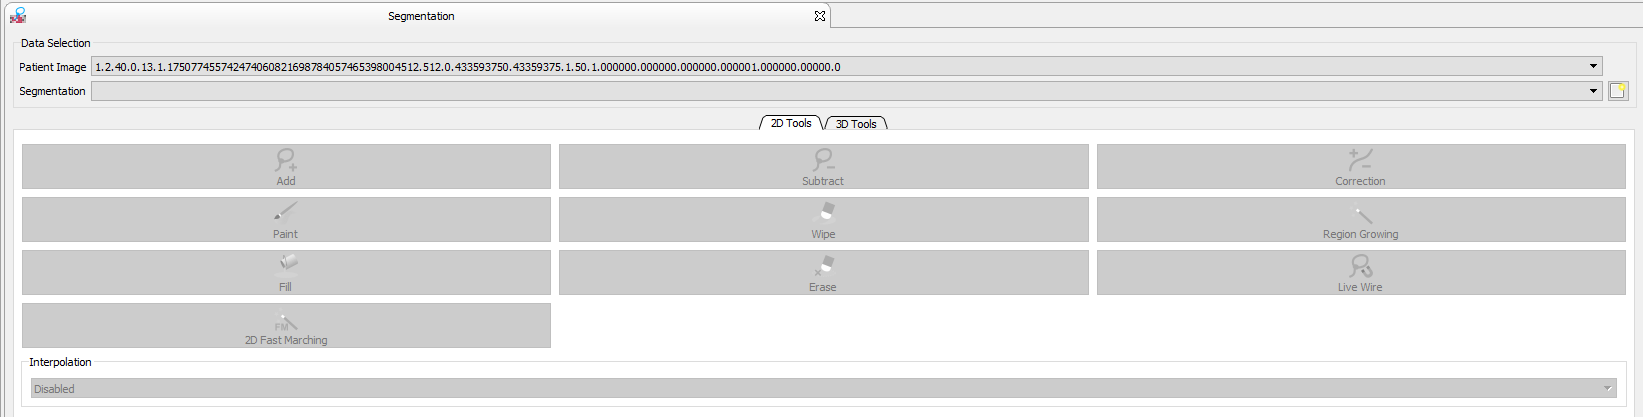
\includegraphics[width=0.7\textwidth]{Logos/MITK_Doku/5.PNG}
\caption{5} 
\label{fig:fuenf} 
\end{figure}

Hat man dies getan, kann das 3D Tool \textit{Region Growing 3D} ausgewählt werden.

\begin{figure}[H] 
\centering 
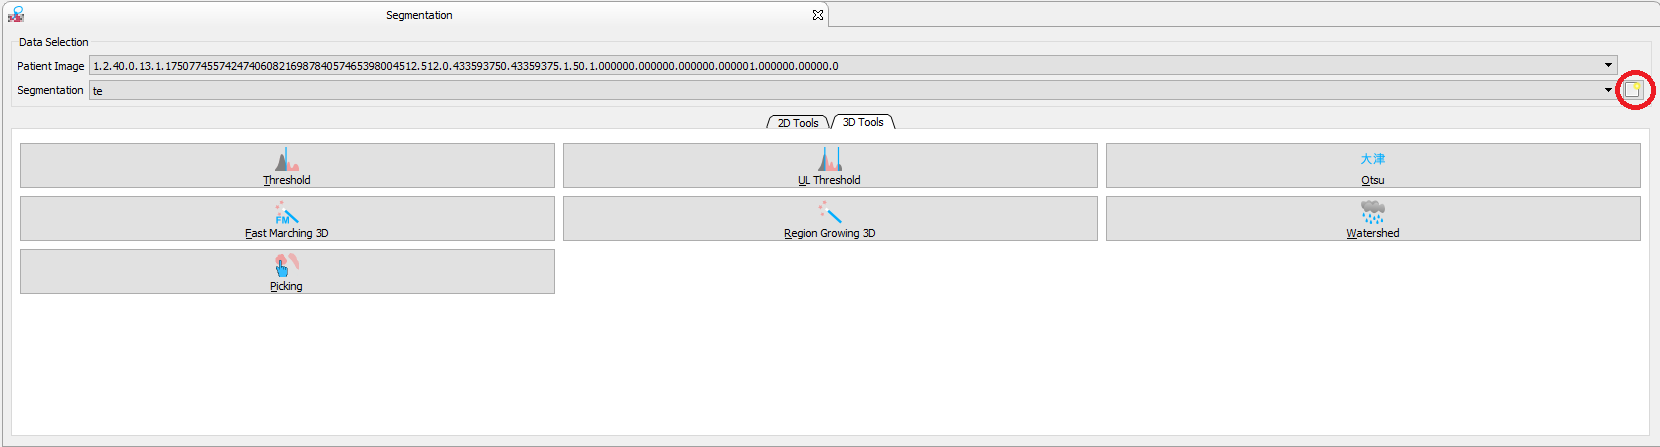
\includegraphics[width=0.7\textwidth]{Logos/MITK_Doku/6.PNG}
\caption{6} 
\label{fig:sechs} 
\end{figure}

Anschließend kann mit Shift + Linke Maustaste eine Punkt im Volumen ausgewählt werden. Danach muss mit  \textit{Run Segmentation} die Segmentierung ausgeführt werden.

\begin{figure}[H] 
\centering 
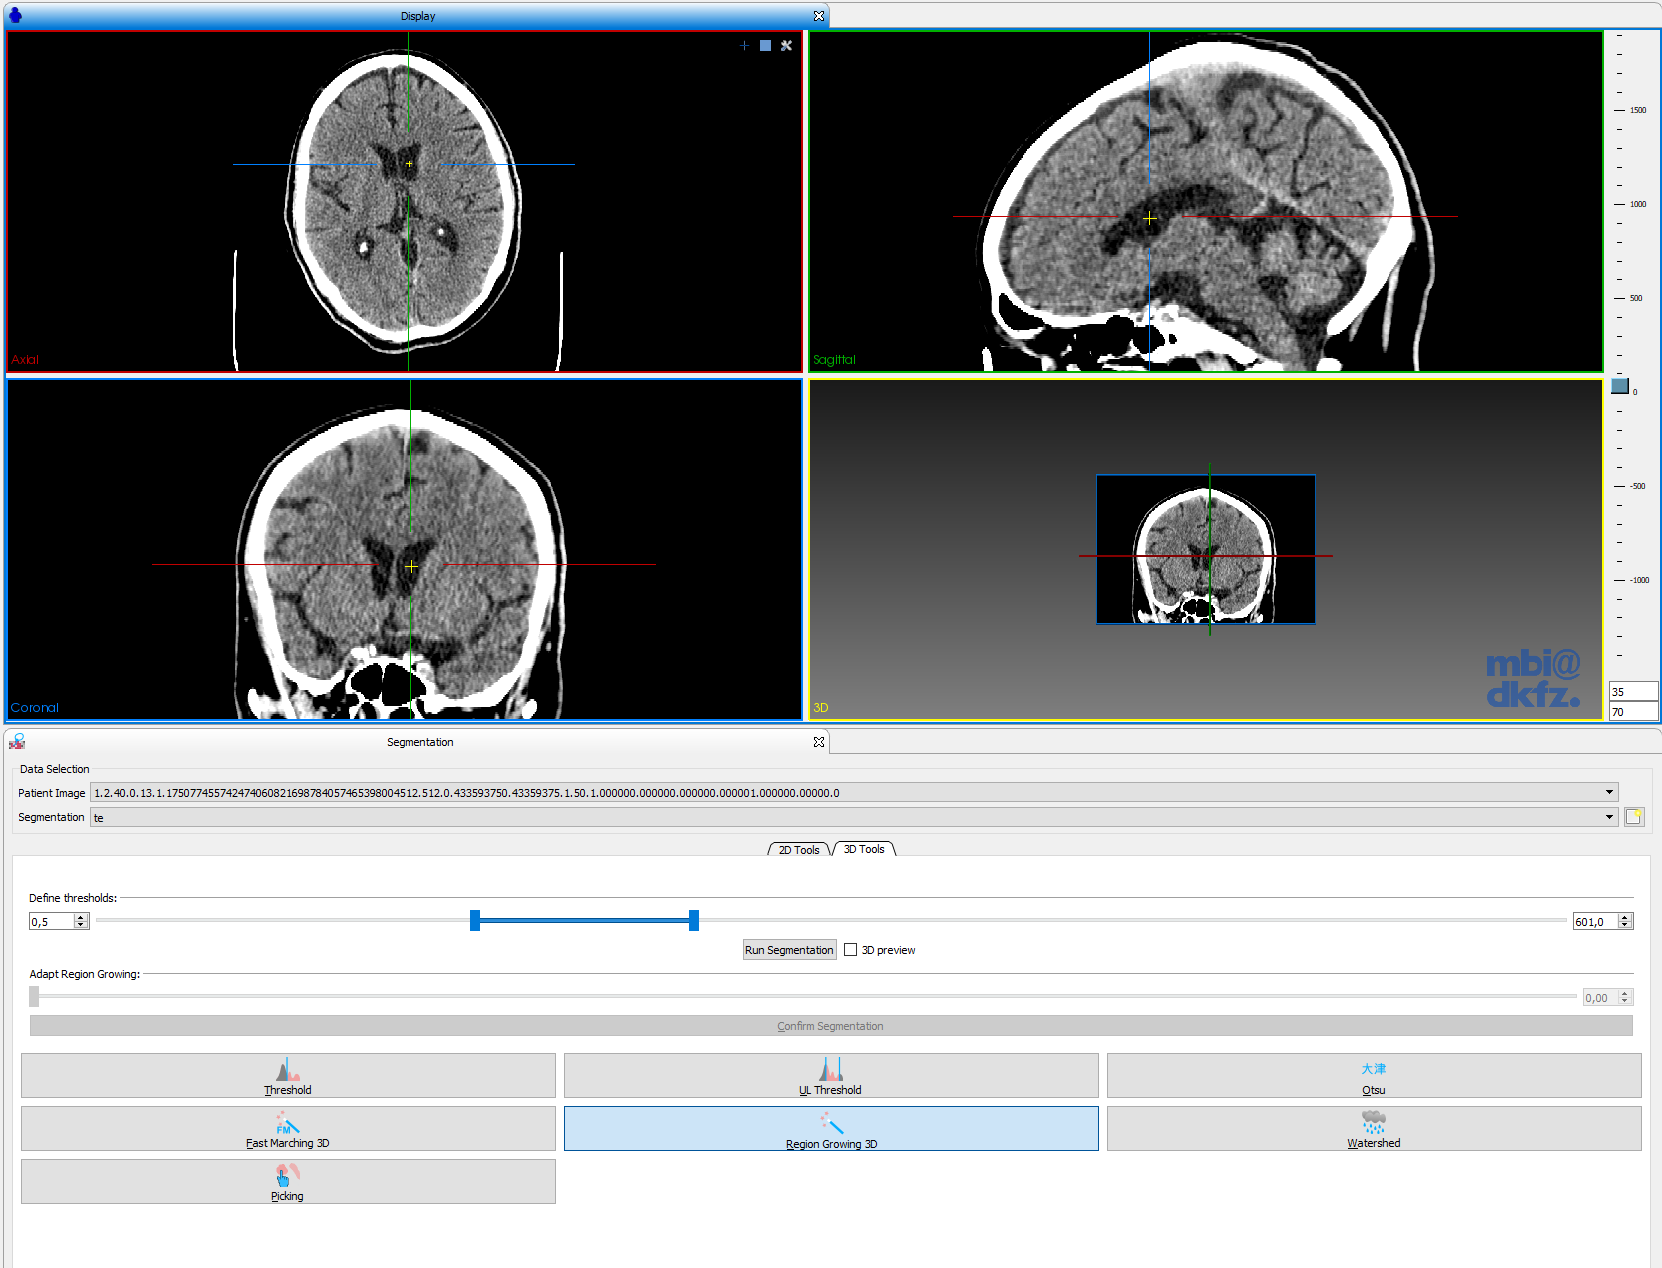
\includegraphics[width=0.7\textwidth]{Logos/MITK_Doku/7.PNG}
\caption{7} 
\label{fig:sieben} 
\end{figure}

Nun kann der Threshhold angepasst und das Region Growing mit dem \textit{Adapt Region Growing} Regler angepasst werden. Wird das gezielte Ergebnis erwünscht, kann es mit \textit{Confirm Segmentation} bestätigt werden.

\begin{figure}[H] 
\centering 
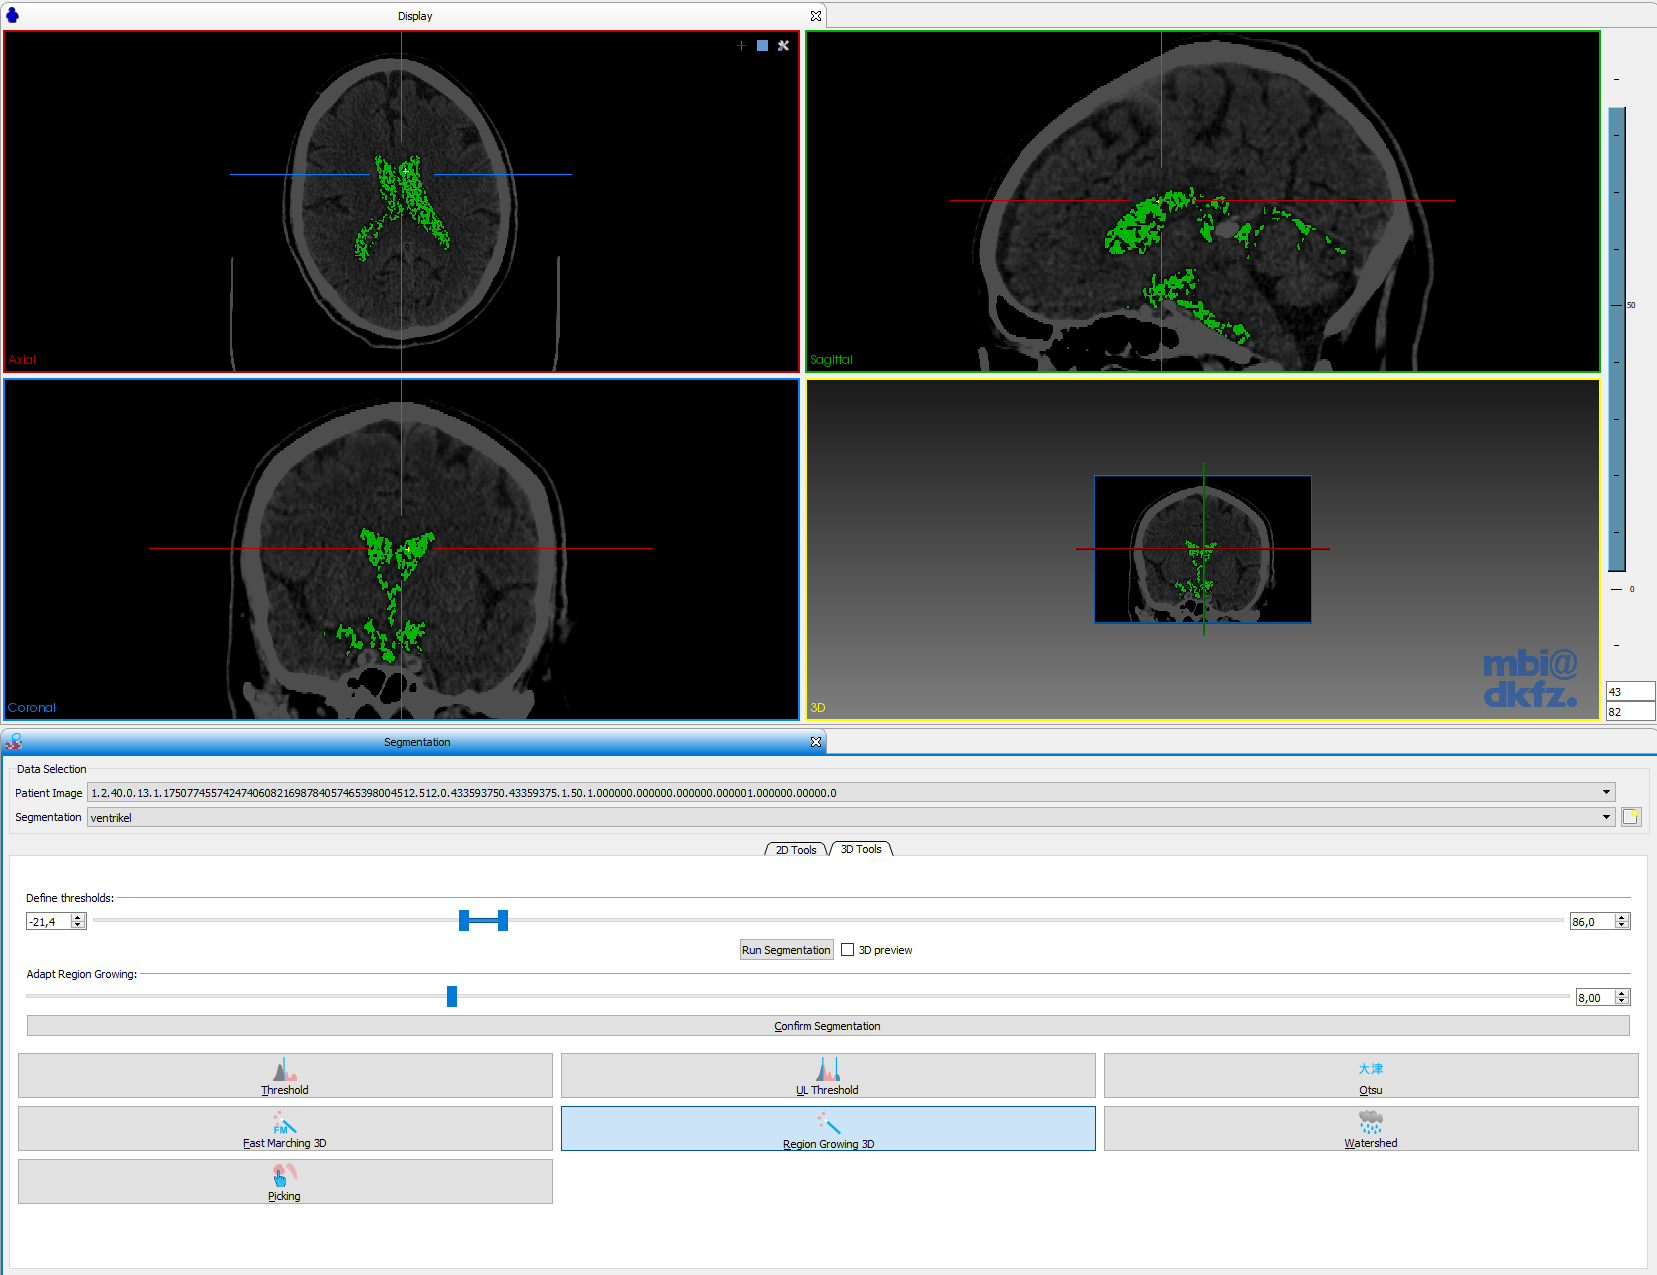
\includegraphics[width=0.7\textwidth]{Logos/MITK_Doku/8.PNG}
\caption{8} 
\label{fig:acht} 
\end{figure}

Mit Tool Nummer 4 kann das Ergebnis mit verschiedenen Operationen verbessert werden. Hierbei wird oft \textit{Closing} benutzt. Anschließend kann mit Rechtsklick auf die Segmentierung im \textit{Data Manager} der Befehl \textit{Create smoothed polygon model} ausgeführt werden

\begin{figure}[H] 
\centering 
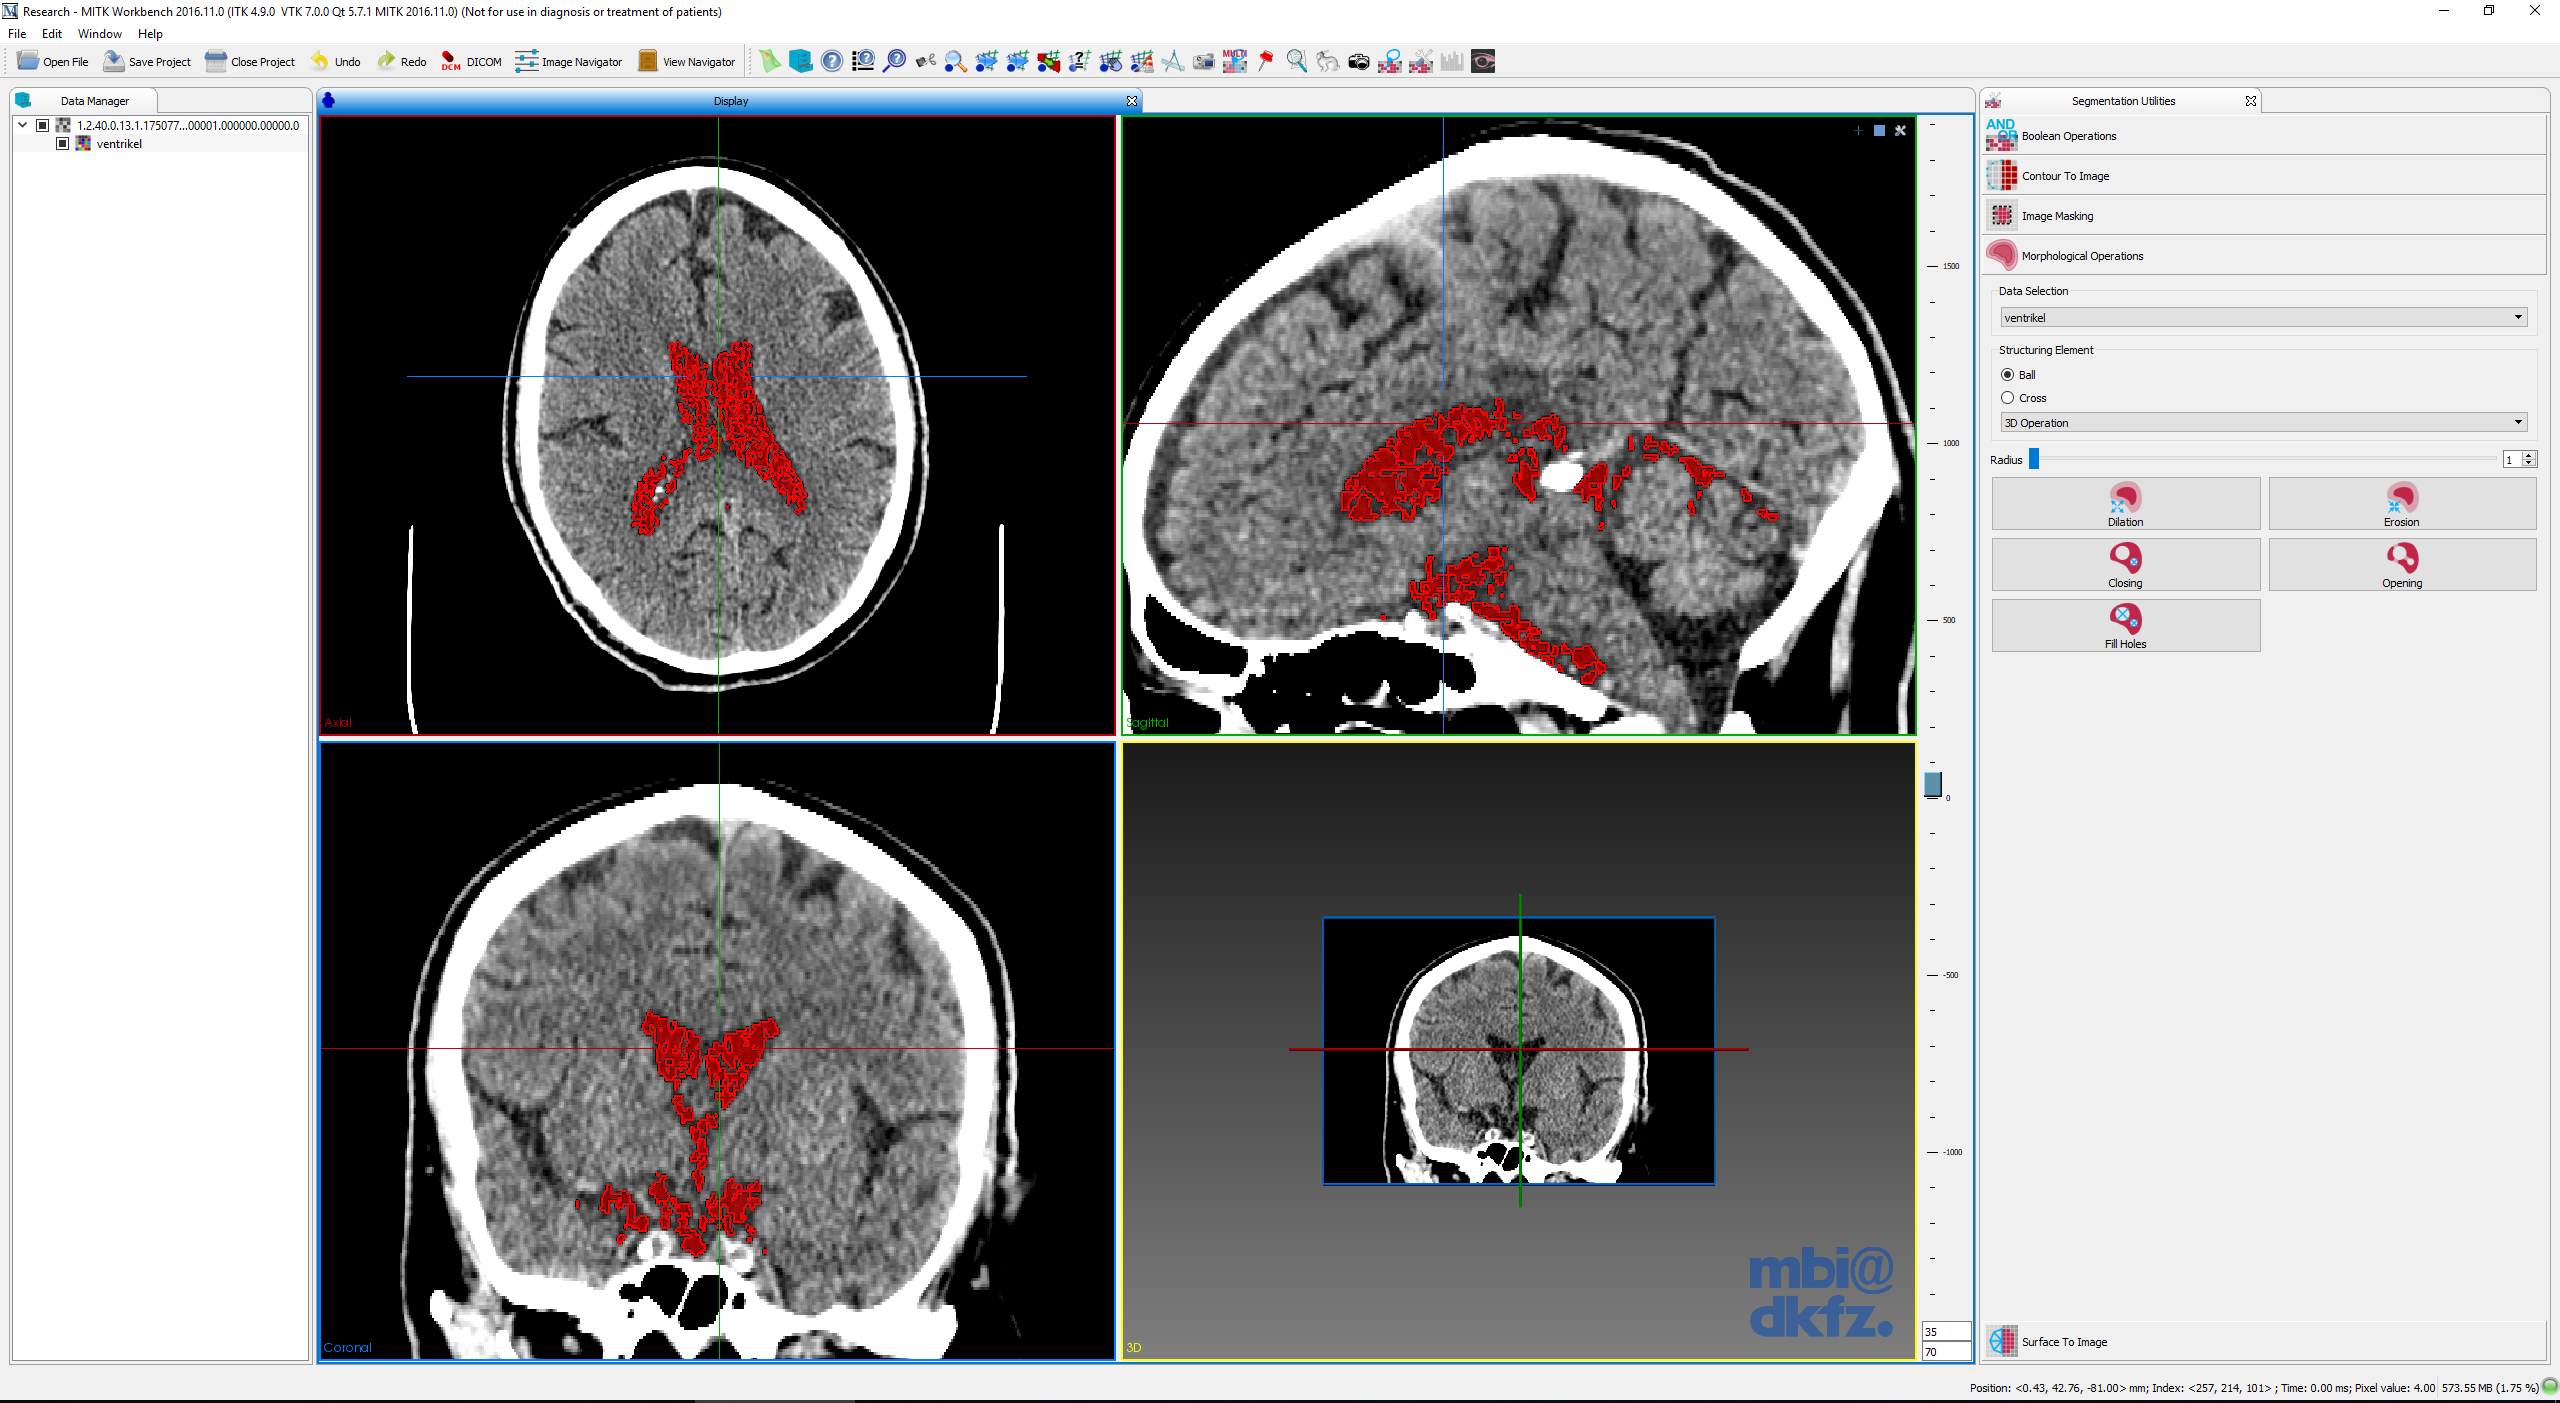
\includegraphics[width=0.7\textwidth]{Logos/MITK_Doku/9.PNG}
\caption{9} 
\label{fig:neun} 
\end{figure}

Nachdem alle diese Schritte befolgt wurden kann man im linken Unteren Kasten die Segmentierung sehen. Mit Tool 5 kann die Darstellung der Segmentierung verändert werden.

\begin{figure}[H] 
\centering 
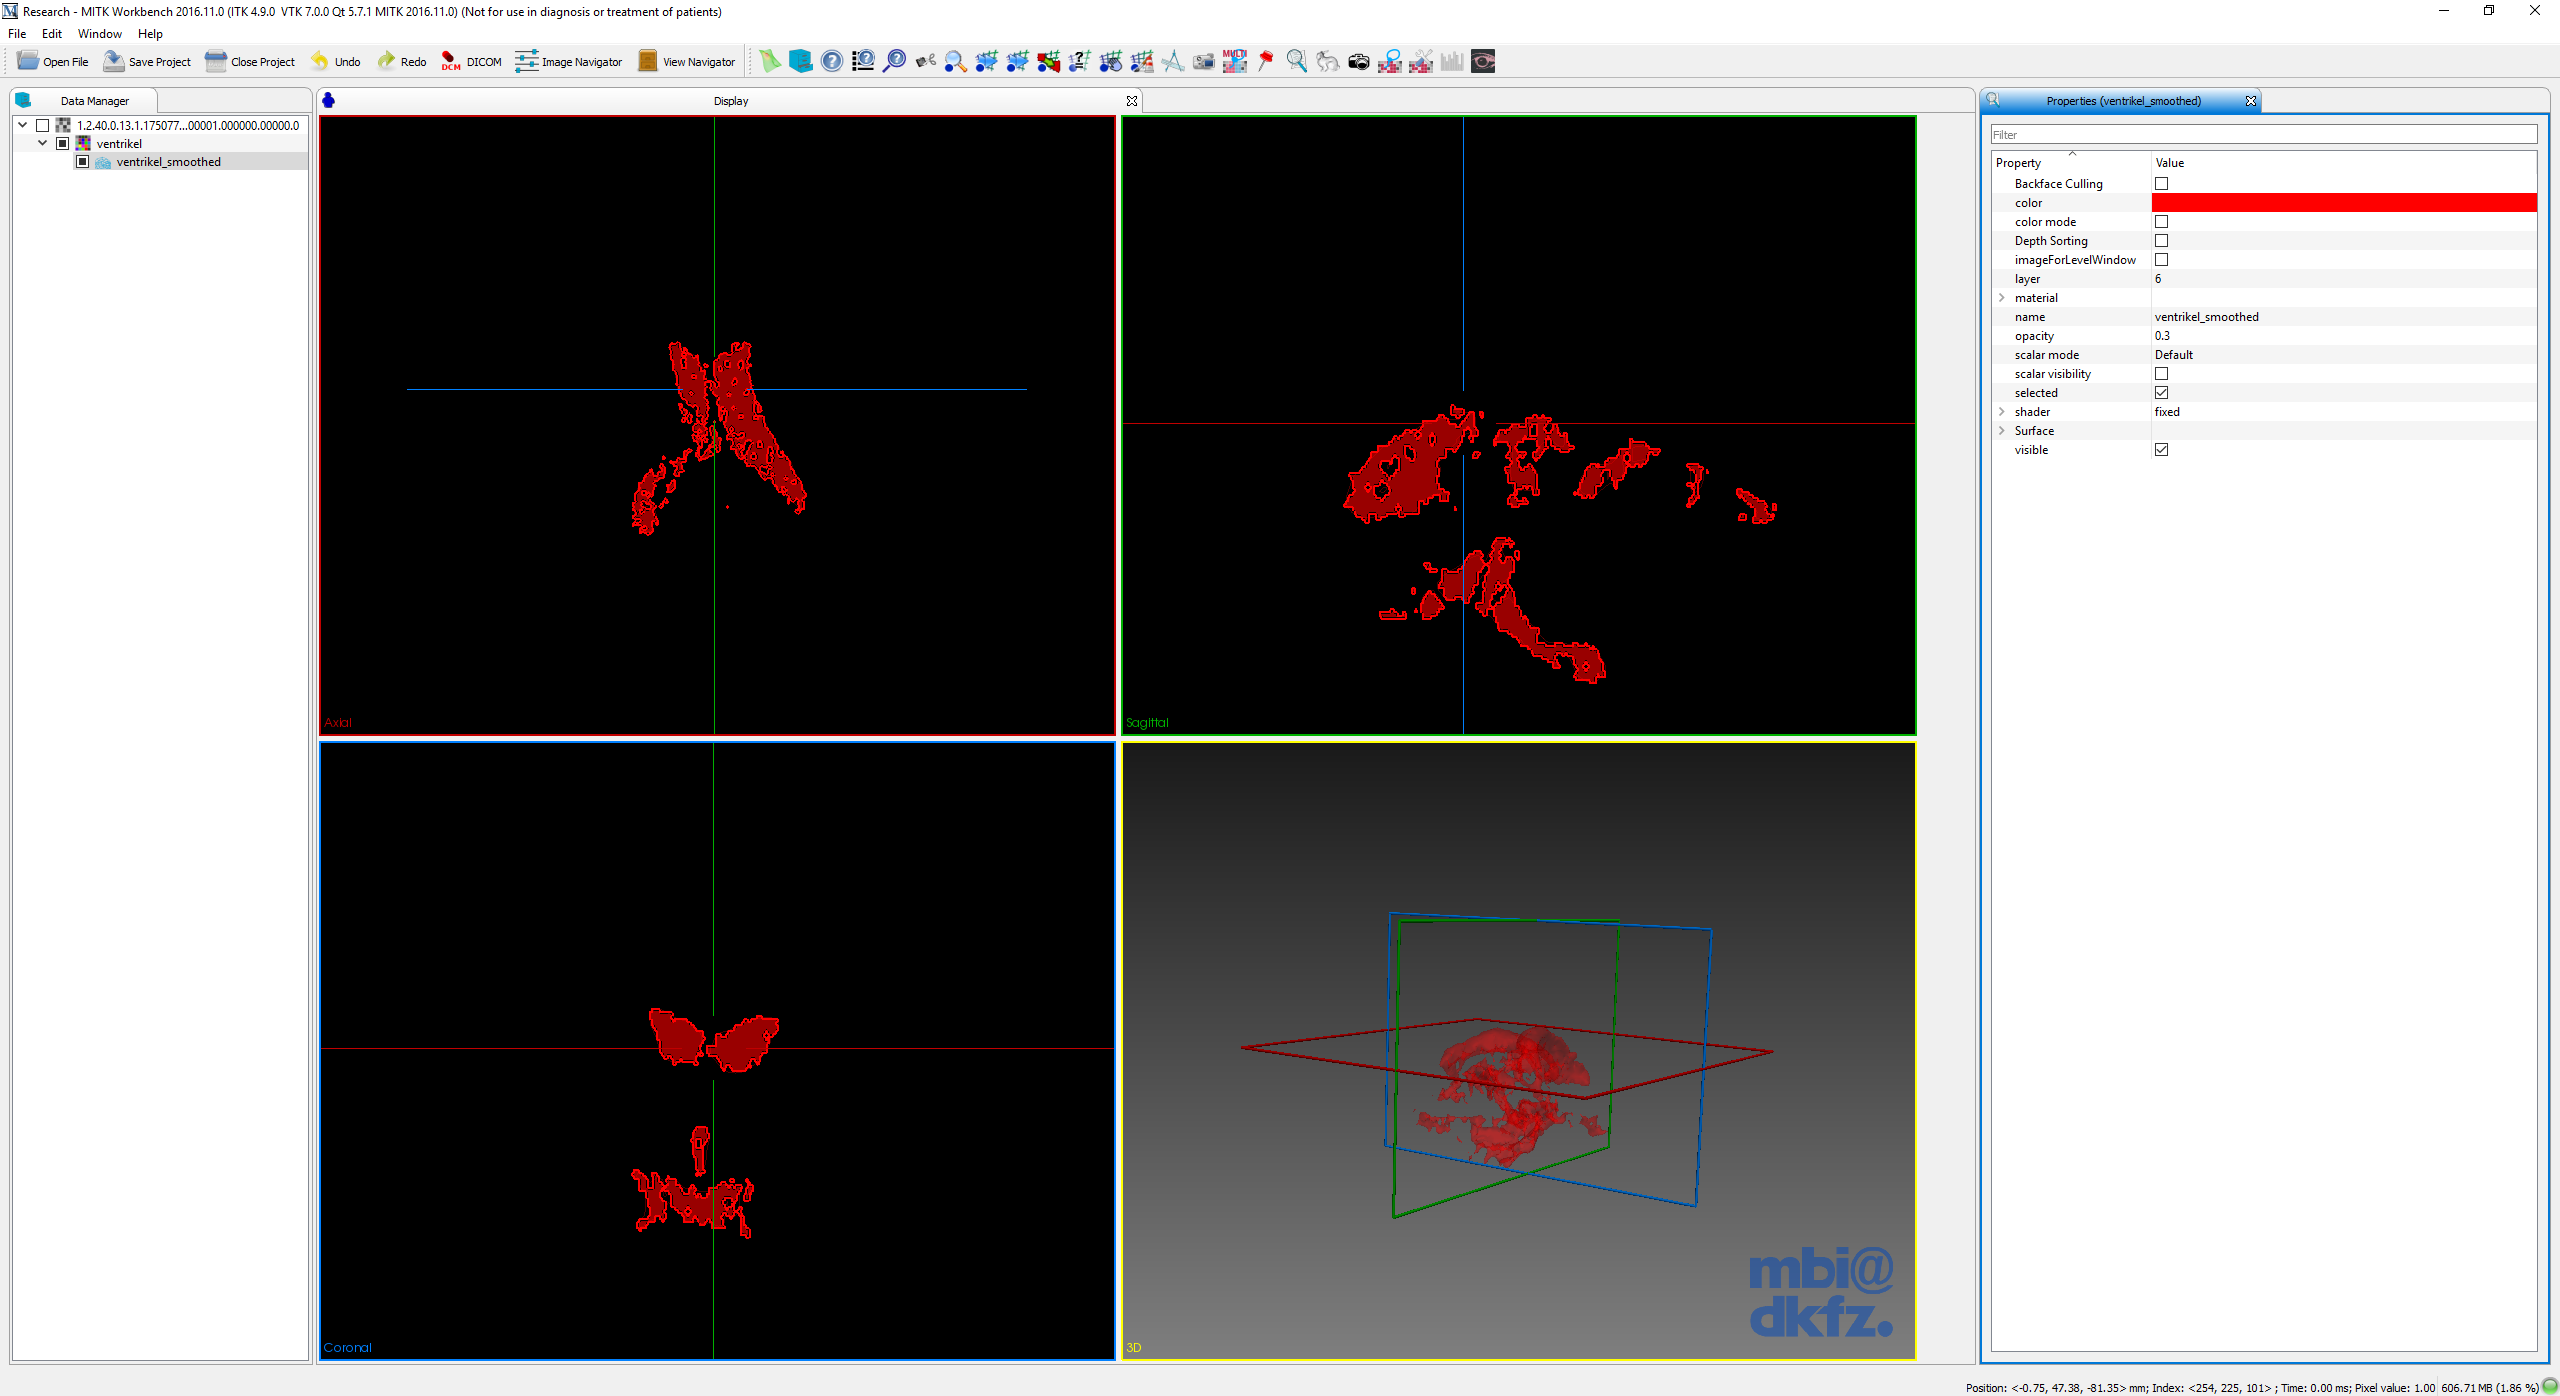
\includegraphics[width=0.7\textwidth]{Logos/MITK_Doku/10.PNG}
\caption{10} 
\label{fig:zehn} 
\end{figure}